\section{Problem Statement}

Sensorimotor Rhythms (SMRs) are specific neural oscillations that occur in the brain's sensorimotor cortex, an area of the brain involved in the planning, controlling, and executing motor functions \cite{leeuwis2021functional}. These rhythms manifest as changes in electrical activity, specifically within the frequency range of approximately 4 to 40 ($Hz$), when an individual performs motor actions or even imagines performing these actions \cite{cattai2021phase}. These changes can be recorded using EEG signals, providing the foundation for non-invasive BCI systems \cite{altaheri2023deep}. One of the most important phenomena associated with SMRs is their synchronization during MI tasks \cite{belwafi2020effective}. This synchronization serves as a unique feature of the specific motor action an individual is imagining or executing \cite{zapala2020effects}. Several methodologies leverage this critical concept to categorize MI tasks \cite{brusini2021systematic}. For instance, Band-power features are based on the idea that SMR synchronization occurs within specific frequency bands such as mu (8-13 Hz) and beta (13-30 Hz) \cite{luo2020motor}. Consequently, they calculate the power of EEG signals within these frequency bands at each electrode at the sensorimotor region. However, it has been proven that synchronization is not necessarily confined to the sensorimotor cortex \cite{singh2021comprehensive}. Among the approaches that consider information from different brain areas, the Common Spatial Patterns (CSP) method is one of the most relevant \cite{yang2021multi}. CSP aims to maximize the separability of SMR features by identifying spatial filters that escalate the variance of relevant SMRs within different MI cognitive processes while reducing the variance of unrelated ones \cite{gaur2021sliding}. These filters are then applied to EEG signals to extract discriminative features for classification. Nevertheless, the temporal evolution of SMR synchronization patterns within the same subject is complex, and simple covariance estimation typically fails to uncover MI tasks \cite{darvish2021correlation}. 

Cognitive processes often activate multiple brain areas that communicate with each other. Specifically, the execution or imagination of simple motor tasks requires the interconnection of multiple cortical regions for information exchange \cite{leeuwis2021functional}. Therefore, brain connectivity (BC), which refers to relationships between brain regions, is crucial for understanding basic brain functions and the role of different regions in MI tasks \cite{ismail2020graph}. BC of MI tasks is linked to synchronization mechanisms within (or sometimes between) different SMRs, primarily emerging in the sensorimotor cortex \cite{maksimenko2017macroscopic}. Moreover, it has been established that BC is a superior technique for interpreting data in the context of MI tasks compared to numerous other methods \cite{collazos2023posthoc}. This is because BC goes beyond isolated features and can represent brain connectivity as graphs, enabling researchers to visualize the connections between brain regions \cite{grana2023review}. This visualization capability allows them to identify alterations in brain connectivity associated with neurological disorders or injuries \cite{lim2021post}. BC also assists in diagnosing conditions, monitoring progress, and tailoring treatment strategies by tracking how patterns evolve during recovery, therapy, or disease progression \cite{yen2023exploring}. BC analysis offers a comprehensive and interpretable approach to understanding brain dynamics, providing valuable insights into network-level interactions and cognitive processes \cite{tafreshi2019functional, van2014functional, sakkalis2011review}. Research into brain connectivity has primarily utilized three types of brain connectivity: structural connectivity (SC), effective connectivity (EC), and functional connectivity (FC). Each of those serves unique purposes in understanding brain activity \cite{cao2022brain}. 

SC focuses on physical connections between different brain regions, typically investigated using diffusion tensor imaging techniques \cite{yeh2021mapping}. While valuable for understanding the brain's underlying architecture, SC cannot be directly estimated using merely EEG techniques \cite{thiebaut2020brain}. Moreover, it fails to capture the dynamic changes during MI tasks, rendering it less suitable for MI-BCI systems \cite{yeh2021mapping}. On the other hand, EC explores the causal influence or directed information flow between brain regions, aiming to uncover directional relationships and determine how one region influences another \cite{cao2022brain}. Dynamic causal modeling \cite{lee2020predicting} and Granger causality \cite{hejazi2019prediction} are useful for inferring causal relationships. Still, they are limited for EEG-based MI-BCI primarily due to their complexity, computational demands, and the need for a priori assumptions \cite{chiarion2023connectivity}. Lastly, FC measures the statistical dependencies or correlations in neural activity between different brain regions. It provides information about synchronized or co-activated regions, highlighting the dynamic changes in brain interactions during MI tasks \cite{friston2011functional}. Although FC might exhibit variability with a limited number of samples, its simplicity, low computational demands, and lack of need for prior assumptions make it particularly well-suited for MI-BCI \cite{hamedi2016electroencephalographic,he2019electrophysiological,sakkalis2011review}.

This thesis will focus its attention on the next critical challenges for EEG-FC-based MI-BCI, which will be discussed in depth further. Firstly, despite the valuable insights derived from standard Functional Connectivity (FC), it faces a performance deficit in MI classification tasks due to the inherently high noise in the EEG signals, issues of volume conduction, and notable inter-subject variability. Second, the heavy reliance on subject matter experts in FC-based feature extraction affects the system's efficiency. This dependence is amplified in scenarios where the same MI cognitive task generates various neural responses in different trials from the same subject, leading to poor and inconsistent predictions. Lastly, the call for model interpretability resonates throughout FC-based MI-BCI systems. With many models functioning like 'black boxes,' providing predictions without clear justifications, achieving a trustworthy, causative, and interactive model that can explain why certain predictions are chosen over others is crucial.

\subsection{Performance Deficit in FC-based MI-BCI Systems}

\textbf{perfromance es un efecto de la incapacidad de calcular connectividades funcionales queue permitan soportar no nonlinear, no stationary and inter subject variability}

While standard FC provides invaluable insights for interpreting brain activity patterns, it often struggles to achieve high accuracy in MI classification tasks \cite{chiarion2023connectivity}. This accuracy issue is especially highlighted when compared with conventional methods like CSP \cite{yang2021novel}. FC quantifies the statistical dependencies between EEG channels, and its accuracy is heavily influenced by challenges such as a low signal-to-noise ratio, volume conduction problems, and inter-subject variability \cite{abiri2019comprehensive,bastos2016tutorial}.

The inherent noise in EEG signals significantly hinders the underlying neural activity, challenging decoding EEG signals \cite{hata2016functional}. Specifically, endogenous and exogenous artifacts, such as electromagnetic interferences, movement artifacts, and individual differences in skull thickness and conductivity can diminish the fidelity of EEG signals~\cite{nentwich2020functional}. As a result, a low signal-to-noise ratio impedes attaining competitive performance. Moreover, functional activities recorded using EEG show volume conduction problems even before they can be measured on the scalp's surface, causing several EEG channels to be correlated \cite{varone2021machine}. This increases the complexity and decreases the precision of the data, especially when measuring functional connectivity where spurious connectivities can be observed \cite{bakhshayesh2019detecting}.

Aside from these issues, individual brain activity's intrinsic diversity and complexity also lead to notable inter-subject variability \cite{wriessnegger2020inter}. Even when different individuals imagine performing the same motor task, their brain connectivity patterns differ, leading to varied SMR synchronization patterns~\cite{wriessnegger2020inter, xie2020review}. For instance, Factors ranging from demographic variables like gender and age to neurophysiological and psychological conditions and individual lifestyle choices result in unstable MI-BCI performance \cite{antonakakis2020inter, huang2023discrepancy}.

Most of the existing FC estimation methods are based on covariance matrices calculated from the original EEG signal domain and do not account for brain activity's inherent nonlinearity and non-stationarity, inevitably compromising their accuracy \cite{miladinovic2021effect}. Moreover, the high variance in brain activity during task execution adds further difficulties in identifying relevant feature patterns. While improvements in covariance matrices estimation might be achieved through mapping and regularization techniques, selecting an appropriate distance metric to encapsulate variability remains challenging \cite{wang2020diverse,congedo2017fixed}.

In summary, implementing and utilizing FC-based MI-BCI systems must overcome significant challenges. Enhancing the model's accuracy without compromising its interpretability is critical. Alongside this, there is a need for innovative strategies that can effectively manage the complex issue of low signal-to-noise ratio, volume conduction problems, and inter-subject variability. \cref{fig:problem_1} shows a representation of these challenges.

\begin{figure}[!h]
    \centering
    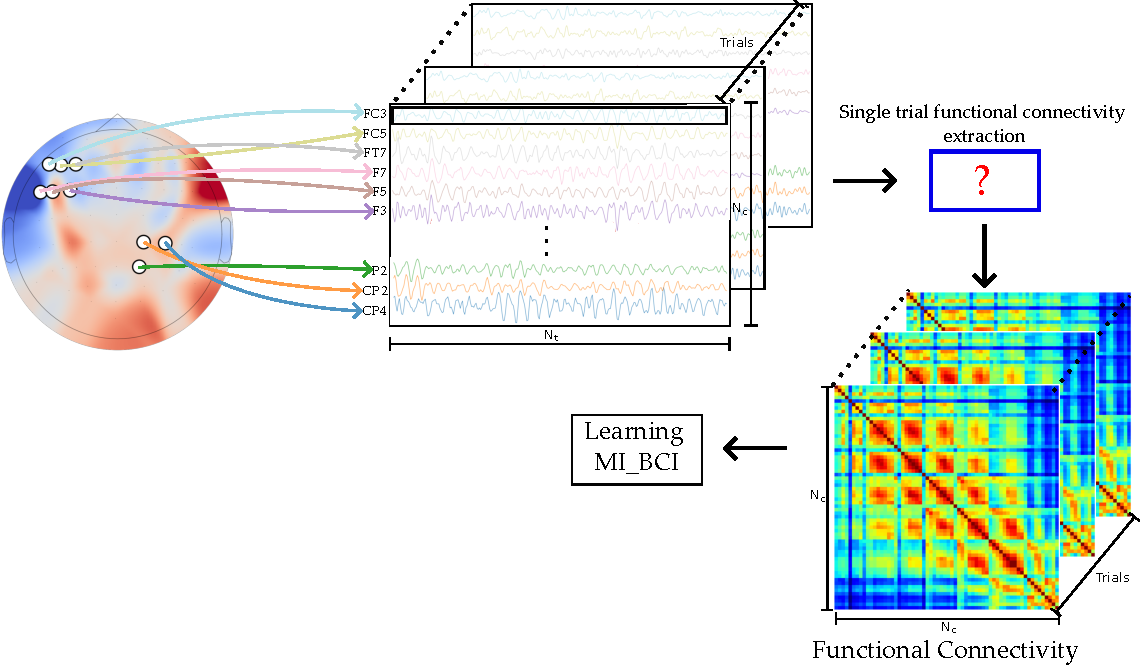
\includegraphics[width=0.9\linewidth]{Figures/Objective_1/problem1.pdf}
    \caption{single-trial functional connectivity graphical scheme}\label{fig:problem_1}
\end{figure}

\subsection{Necessity of Subject Matter Experts in FC-based Feature Extraction}

Despite substantial advancements in classical MI-BCI systems, decoding EEG signals remains a significant challenge \cite{rashid2020current}. For instance, functional connectivity analysis is intricate due to the nonlinear correlation of signals across EEG channels, which poses a particular challenge for conventional MI-EEG methods, especially in improving low-performing individual accuracy \cite{ismail2020graph,wang2020diverse,congedo2017fixed}. The complexities are further compounded by the handcrafted feature extraction steps, leading to potential high information loss and a persistent low signal-to-noise ratio, thereby limiting the ability to find discriminative correlations between EEG channels \cite{altaheri2023deep}.

Feature extraction from raw EEG data, such as selecting proper band filters, heavily depends on human expertise \cite{chamola2020brain, padfield2019eeg}. Although subject matter experts can help derive relevant features, their knowledge often proves insufficient, especially when a subject produces different SMRs for the same MI cognitive task across different trials within a single subject\cite{altaheri2023deep, vidaurre2020sensorimotor}. Further complexity that potentially impedes effective feature extraction from raw EEG signals is introduced as additional concurrent cognitive processes, such as fatigue, visual stimuli, or other cognitive tasks \cite{saha2020intra, ismail2020graph, meers2020motor, talukdar2019motor}.

In summary, extracting relevant features from raw EEG data for use in FC-based MI-BCI systems presents considerable challenges, primarily arising from the complexity of EEG data and the heavy reliance on subject matter experts. While various filter bank methods have been proposed, there is a pressing need for automated end-to-end feature extraction approaches that can automatically model and adjust to subject-specific sub-band filters. \cref{fig:problem_2} visually illustrates these challenges.


\begin{figure}[!h]
    \centering
    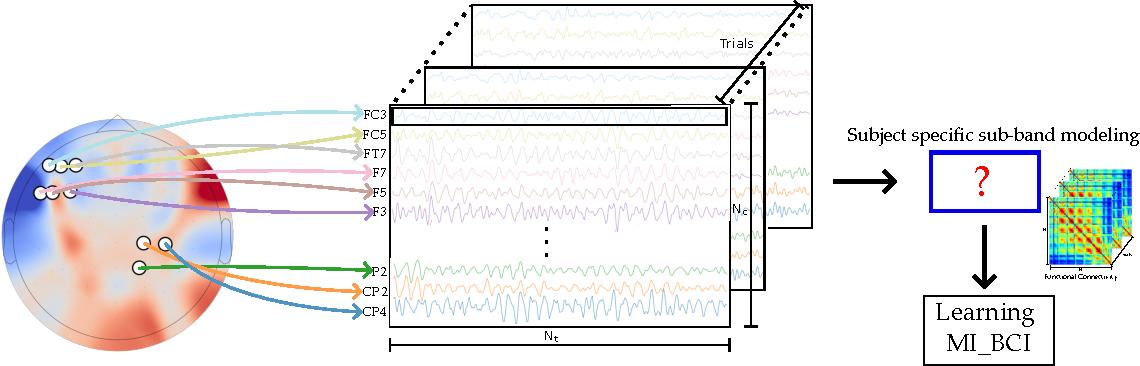
\includegraphics[width=0.9\linewidth]{Figures/Objective_2/problem2.pdf}
    \caption{Sub-band modeling graphical scheme}\label{fig:problem_2}
\end{figure}


\subsection{Call for Model Interpretability in FC-based MI-BCI Systems}

The third pressing challenge in FC-based MI-BCI systems is the need for model transparency. This requirement echoes the fundamental goal of Explainable AI (XAI), which is yielding pertinent insights into the mechanisms behind model predictions, thereby fostering characteristics such as trustworthiness, causality, transferability, confidence, accessibility, and interactivity \cite{smuha2019eu}. This challenge gains unique complexity in the context of integrating various sub-frequency bands in MI-BCI systems \cite{guillot2019benefits}. Often, these sophisticated models function like 'black boxes,' providing results without explanations or justifications \cite{ras2018explanation}, as shown in \cref{fig:problem_3}.

Understanding why a model prefers certain predictions over others extends beyond predictive efficacy, especially in critical domains such as health and medical decision-making \cite{miotto2018deep}. Interpretation should highlight which features get prioritized during model training and demonstrate how feature correlations influence such decisions \cite{zeiler2014visualizing, chakraborty2017interpretability}. As model refinement enhances performance, the need for transparency and interpretability grows, particularly in clinical research settings where reliance on model recommendations is paramount \cite{xiao2018opportunities}.

Additionally, defining 'interpretability' remains controversial, giving rise to various interpretation methodologies \cite{fan2021interpretability}. In the context of FC-based end-to-end sub-band modeling in MI-BCI, the challenge involves developing an interpretability framework that consolidates the individual contributions of each frequency band towards classification across different MI tasks \cite{zuk2020eeg}. Notably, detecting the inclusion of irrelevant features, particularly those arising from noisy functional connectivity patterns, is vital for refining the model, increasing its generalization, reducing overfitting risks, and furthering the use of MI-BCI within clinical applications like diagnosis, monitoring, and computer-assisted learning \cite{qian2018brain}.


\begin{figure}[!h]
    \centering
    \includegraphics[width=0.9\linewidth]{Figures/Objective_3/problem3.pdf}
    \caption{BCI MI model interpretability graphical scheme}\label{fig:problem_3}
\end{figure}